\documentclass[a4paper,10pt]{article}
\usepackage[utf8]{inputenc}

\usepackage[labeled,resetlabels]{multibib}
\usepackage[binary-units]{siunitx}
\sisetup{group-separator={,},
     detect-all,
     binary-units,
     list-units = single,
     range-units = single,
     range-phrase = --,
     per-mode = symbol-or-fraction,
     separate-uncertainty = true,
     multi-part-units = single,
     list-final-separator = {, and }
%    scientific-notation = fixed
}

\usepackage{amsmath}
\usepackage{caption}
\usepackage{subcaption}
\usepackage{booktabs,multirow}
\usepackage{floatrow}
\usepackage{graphicx}
\usepackage{hyperref}
\usepackage[nameinlink]{cleveref}
\usepackage{xcolor}
\hypersetup{
    colorlinks,
    linkcolor={blue!50!black},
    citecolor={red!50!black},
    urlcolor={blue!80!black}
}

\usepackage{todonotes}

\newcites{S}{Selected Bibliography}
\newfloatcommand{capbtabbox}{table}[][\FBwidth]

\def\avx/{\texttt{avx2}}
\def\sse/{\texttt{sse4.2}}
\def\gpuold/{\texttt{C2075}}
\def\gpunew/{\texttt{K40m}}

%opening
\title{Accelerating reacting flow simulations via vectorized chemical kinetic evaluation and integration}
\author{Nicholas Curtis}

\begin{document}

\maketitle

\section*{Introduction}
As the combustion community has recognized the importance of detailed chemical kinetics for predictive reactive-flow simulations, chemical kinetic models have grown in size and complexity to describe current and next-generation fuels relevant to transportation and power generation.
Several studies~\cite{Huang20091814,Bottone2012,Moiz2016123} have demonstrated that the chemical kinetic integration of even modestly sized chemical kinetic models can incur severe computation overhead in realistic reactive-flow simulations.
Many techniques to reduce the cost of utilizing detailed chemical models in reactive-flow simulations exist~\cite{LU2009192}; in particular, a carefully derived analytical formulation of the Jacobian matrix can greatly increase sparsity~\cite{SCHWER2002270} and drop the cost of Jacobian evaluation to linearly depend on the number of species in the model~\cite{LU2009192}.
In addition, studies have shown~\citeS{curtis2017investigation,Niemeyer:2016aa}\cite{STONE201818} that Single-Instruction, Multiple-Data (SIMD) and the related Single-Instruction, Multiple-Thread (SIMT) processors can accelerate chemical kinetic simulations through vectorized evaluation.

This work details efforts to develop and validate open-source algorithms to accelerate integration of stiff chemical kinetic ordinary differential equations (ODEs) via vectorized execution on SIMD and SIMT devices.
This includes codes to evaluate the chemical kinetic source terms and a sparse, analytical Jacobian, as well as ODE integration algorithms for the CPU, GPU and other accelerators.
The developed algorithms will be applied to a detailed large eddy simulation of a bluff-body stabilized turbulent reacting flame, in order to demonstrate accuracy and computational efficiency.


\section{An investigation of GPU-based stiff chemical kinetics integration methods}
\nociteS{curtis2017investigation}
A fifth-order implicit Runge--Kutta method and two fourth-order exponential integration methods equipped with Krylov subspace approximations were implemented for the GPU and paired with the analytical chemical kinetic Jacobian software \texttt{pyJac}.
The performance of each algorithm was evaluated by integrating thermochemical state data sampled from stochastic partially stirred reactor simulations and compared with the commonly used CPU-based implicit integrator \texttt{CVODE}.
We estimated that the implicit Runge--Kutta method running on a single Tesla C2075 GPU is equivalent to \texttt{CVODE} running on \numrange{12}{38} Intel Xeon E5-4640 v2 CPU cores (\Cref{T:gpu_perf}) for integration of a single global integration time step of \SI{e-6}{\second} with hydrogen and methane kinetic models.
In the stiffest case studied---the methane model with a global integration time step of \SI{e-4}{\second}---thread divergence and higher memory traffic significantly decreased GPU performance to the equivalent of \texttt{CVODE} running on approximately three CPU cores.
The exponential integration algorithms performed more slowly than the implicit integrators on both the CPU and GPU.
Thread divergence and memory traffic were identified as the main limiters of GPU integrator performance, and techniques to mitigate these issues were discussed.
Use of a finite-difference Jacobian on the GPU---in place of the analytical Jacobian provided by \texttt{pyJac}---greatly decreased integrator performance (\Cref{F:fd_jac}) due to thread divergence, resulting in maximum slowdowns of \SIrange{7.11}{240.96}{$\times$}; in comparison, the corresponding slowdowns on the CPU were just \SIrange{1.39}{2.61}{$\times$}, underscoring the importance of use of an analytical Jacobian for efficient GPU integration.
Finally, future research directions for working towards enabling realistic chemistry in reactive-flow simulations via GPU\slash SIMT accelerated stiff chemical kinetics integration were identified.

\begin{figure}[htb!]
  %\floatsetup{floatrowsep=qquad}
  \begin{floatrow}
    \capbtabbox{%
    \begin{tabular}{@{}l S[table-format=2.1] S[table-format=2.1] @{}}
      \toprule
      \multirow{2}{*}{$\Delta t$} & \multicolumn{2}{c}{\# equivalent CPU cores} \\ \cmidrule{2-3}
      & {Hydrogen} & {GRI-Mech 3.0} \\
      \midrule
      \SI{e-6}{\second} & 38 & 12 \\
      \SI{e-4}{\second} & 15 & 3 \\
      \bottomrule
    \end{tabular}
    }{%
      \captionsetup{width=0.5\textwidth}
      \caption{Approximate number of CPU cores running \texttt{CVODES} required to match performance of implicit Runge--Kutta algorithm on a single GPU for various models and integration time-step sizes.}%
      \label{T:gpu_perf}
    }%
    \ffigbox[\FBwidth]{%
      \captionsetup{width=0.5\textwidth}
      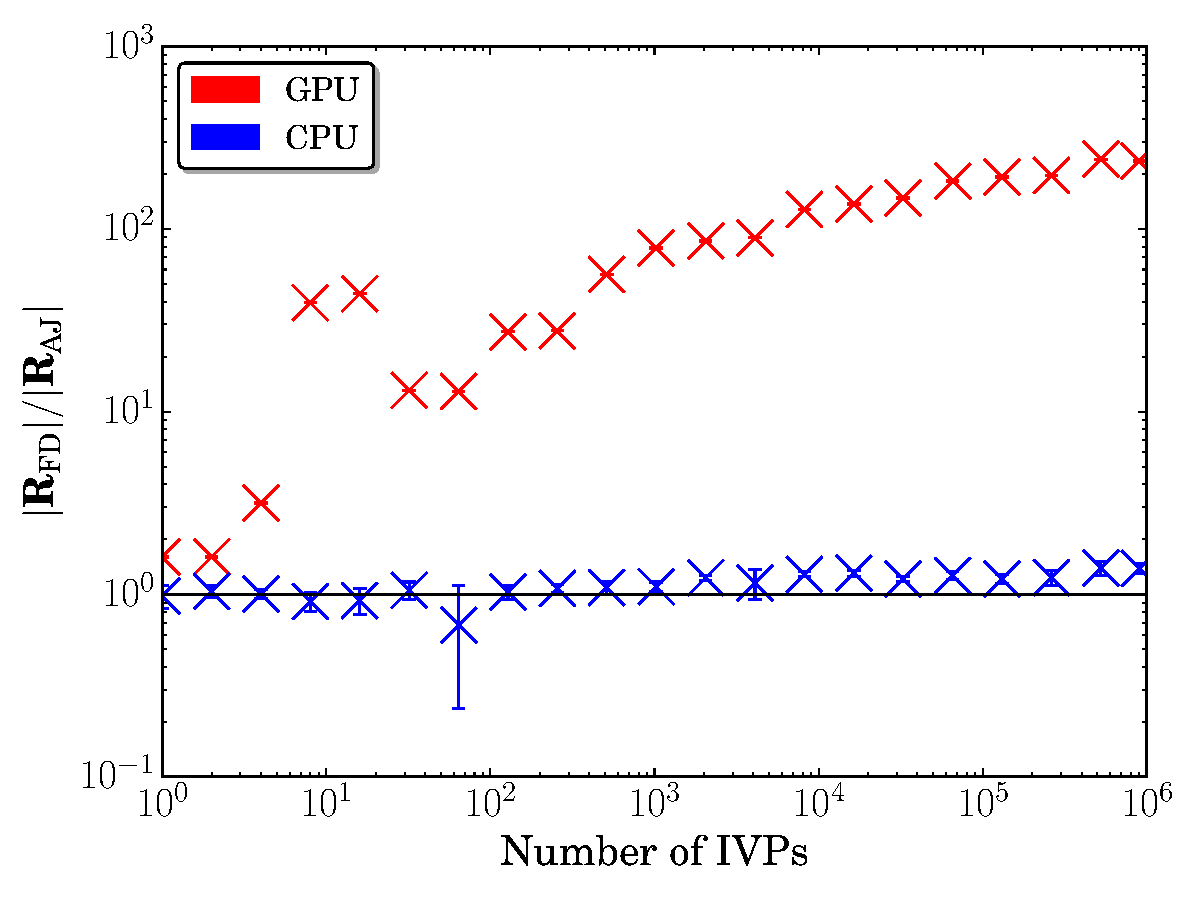
\includegraphics[width=0.5\textwidth]{H2_1e-04_ajac_comp.pdf}
    }{%
      \caption{Ratio of the average finite-difference Jacobian based integrator runtime $\lvert\textbf{R}_{\text{FD}}\rvert$ to that of the analytical Jacobian runtime $\lvert\textbf{R}_{\text{AJ}}\rvert$
	       for the implicit Runge--Kutta (CPU\slash GPU) solvers using the hydrogen model with a global integration step-size of $\Delta t = \SI{e-4}{\sec}$.}
      \label{F:fd_jac}
    }
  \end{floatrow}
\end{figure}

\section{Using SIMD and SIMT vectorization to evaluate sparse chemical kinetic Jacobian matrices and thermochemical source terms}
\nociteS{CURTIS2018186}
Accurately predicting key combustion phenomena in reactive-flow simulations, e.g., lean blow-out, extinction\slash ignition limits and pollutant formation, necessitates the use of detailed chemical kinetics.
The large size and high levels of numerical stiffness typically present in chemical kinetic models relevant to transportation\slash power-generation applications make the efficient evaluation\slash factorization of the chemical kinetic Jacobian and thermochemical source-terms critical to the performance of reactive-flow codes.
Here we investigate the performance of vectorized evaluation of constant-pressure/volume thermochemical source-term and sparse/dense chemical kinetic Jacobians using single-instruction, multiple-data (SIMD) and single-instruction, multiple thread (SIMT) paradigms. These are implemented in pyJac, an open-source, reproducible code generation platform.
Selected chemical kinetic models covering the range of sizes typically used in reactive-flow simulations were used for demonstration.
A new formulation of the chemical kinetic governing equations was derived and verified, resulting in Jacobian sparsities of \SIrange{28.6}{92.0}{$\percent$} for the tested models.
Speedups of \SIrange{3.40}{4.08}{$\times$} were found for shallow-vectorized OpenCL source-rate evaluation compared with a parallel OpenMP code (\Cref{F:source}) on an \avx/ central processing unit (CPU), increasing to \SIrange{6.63}{9.44}{$\times$} and \SIrange{3.03}{4.23}{$\times$} for sparse and dense chemical kinetic Jacobian evaluation (\Cref{F:jac}), respectively.
Furthermore, the effect of data-ordering was investigated and a storage pattern specifically formulated for vectorized evaluation was proposed; as well, the effect of the constant pressure\slash volume assumptions and varying vector widths were studied on source-term evaluation performance.
Speedups reached up to \SI{17.60}{$\times$} and \SI{45.13}{$\times$} for dense and sparse evaluation on the GPU, and up to \SI{55.11}{$\times$} and \SI{245.63}{$\times$} on the CPU over a first-order finite-difference  Jacobian approach.
Further, dense Jacobian evaluation was up to \SI{19.56}{$\times$} and \SI{2.84}{$\times$} times faster than a previous version of \texttt{pyJac} on a CPU and GPU, respectively.
Finally, future directions for vectorized chemical kinetic evaluation and sparse linear-algebra techniques were discussed.


\begin{figure}[!htb]
  \begin{subfigure}[t]{0.45\textwidth}
   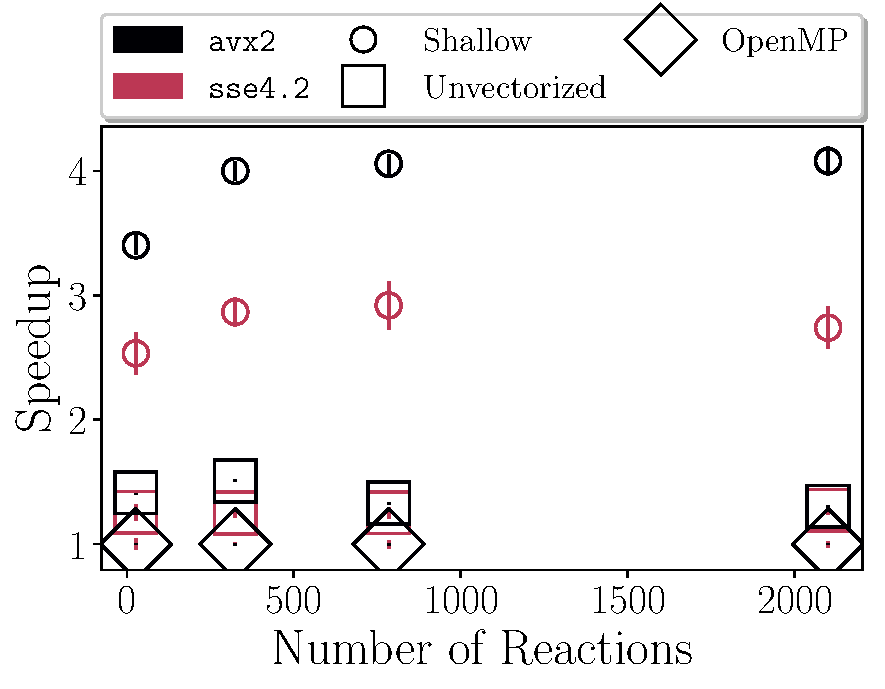
\includegraphics[width=\textwidth]{intel_source.pdf}
   \caption{Speedup of vectorized source-term evaluation over simple parallel evaluation on two different CPUs.}
   \label{F:source}
  \end{subfigure}%
  \qquad
  \begin{subfigure}[t]{0.45\textwidth}
   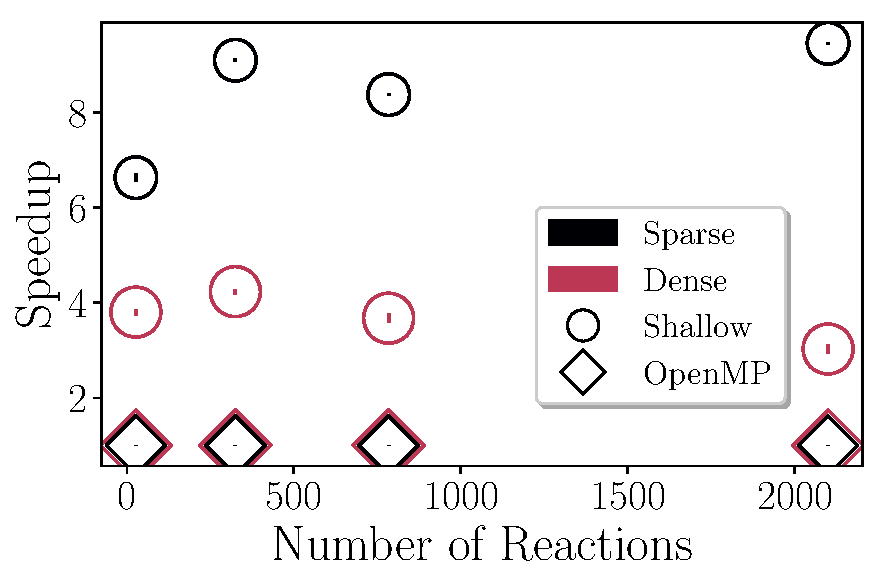
\includegraphics[width=\textwidth]{sparse_vs_dense_speedup.pdf}
   \caption{Speedup of sparse and dense chemical kinetic Jacobian evaluation over simple parallel evaluation on a CPU with \avx/ instructions.}
   \label{F:jac}
  \end{subfigure}
  \caption{Acceleration of chemical kinetic source terms and sparse\slash dense analytical Jacobian on the CPU using \texttt{pyJac-V2}}
\end{figure}



\section{Accelerating large-eddy simulations with SIMD-vectorized chemical kinetic integration}
The Volvo bluff-body premixed turbulent reacting flame~\cite{sjunnesson1991validation,sjunnesson1991lda} was modeled using the OpenFOAM computational fluid dynamics library.
A large eddy simulation was conducted for a non-reacting case, with a \SI{2}{\milli\meter} hexagonal mesh and \SI{0.3}{\milli\meter} wall-normal distance (\Cref{F:mesh}), resulting in roughly \num{2.37e6} total cells.
The non-reacting velocity profiles were validated against experimentally measured mean and fluctuating velocities~\cite{sjunnesson1991validation,sjunnesson1991lda}.
A reacting stoichiometic methane case utilizing the GRI-Mech 3.0 model (\Cref{F:flame}) was then run on \num{96} cores of Intel\raisebox{1ex}{\scriptsize{\textregistered}} Xeon\raisebox{1ex}{\scriptsize{\textregistered}} E5-2690 v3 Processors (four nodes total) with the built-in fourth-order linearly-implicit Rosenbrock integration algorithm present in OpenFOAM (which includes a semi-analytical chemical kinetic Jacobian) to obtain a performance benchmark.
Finally, an open-source, vectorized ODE integration algorithm for the CPU (currently under development)---consisting of a similar linearly-implicit method implemented in OpenCL~\cite{STONE201818}, chemical kinetic source terms, and analytical Jacobian~\citeS{CURTIS2018186}---will be applied to the problem.
The developed algorithm will be compared to the built-in OpenFOAM solver to determine the accuracy, effective speedup and resulting impact on chemistry load-balancing.
Future directions and improvements, including sparse linear-algebra and load-balancing algorithms suited for the vectorized solver will be detailed.


\begin{figure}[!htb]
  \begin{subfigure}[t]{0.45\textwidth}
   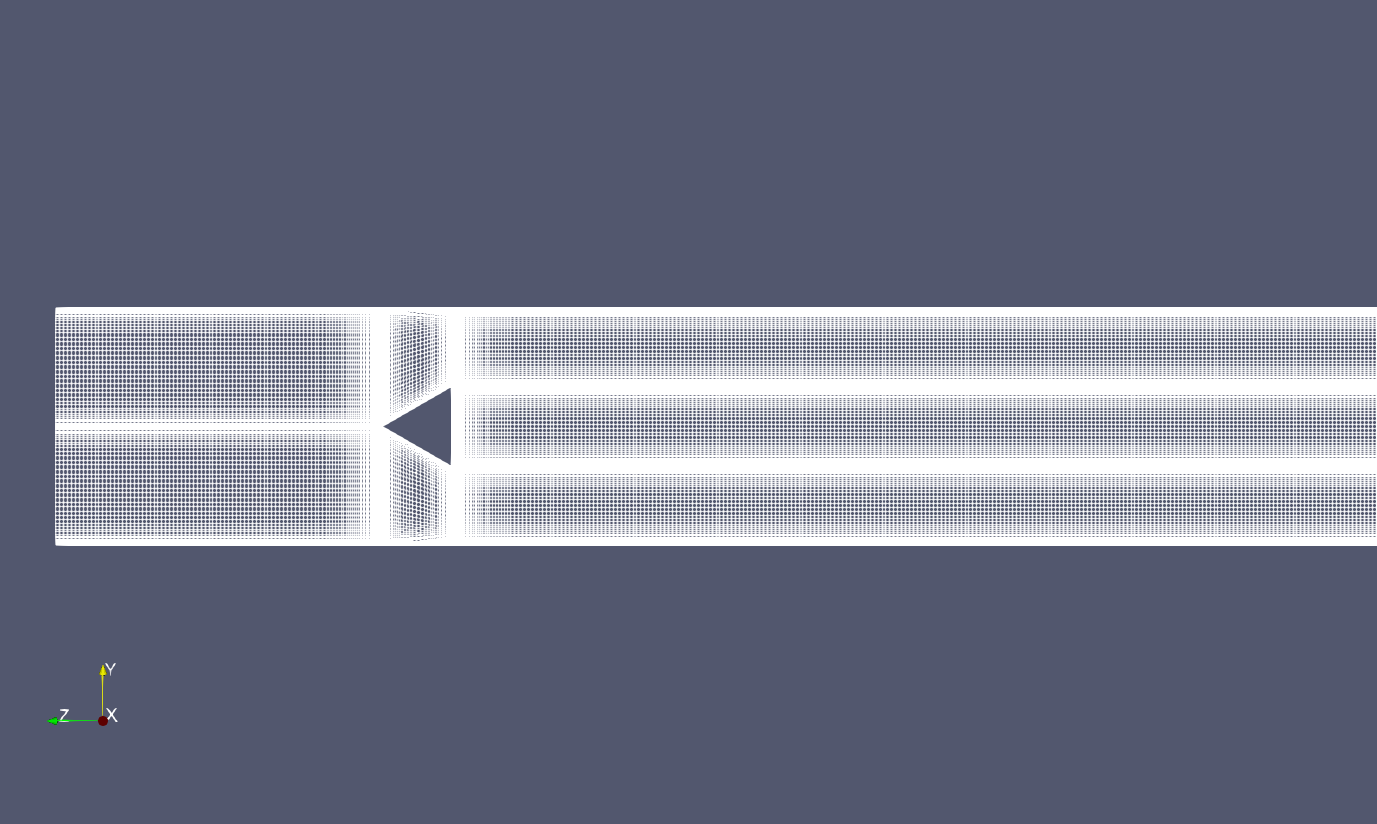
\includegraphics[width=\textwidth]{mesh.png}
   \caption{\SI{2}{\milli\meter} mesh used in bluff-body stabilized flame simulation.}
   \label{F:mesh}
  \end{subfigure}%
  \qquad
  \begin{subfigure}[t]{0.45\textwidth}
   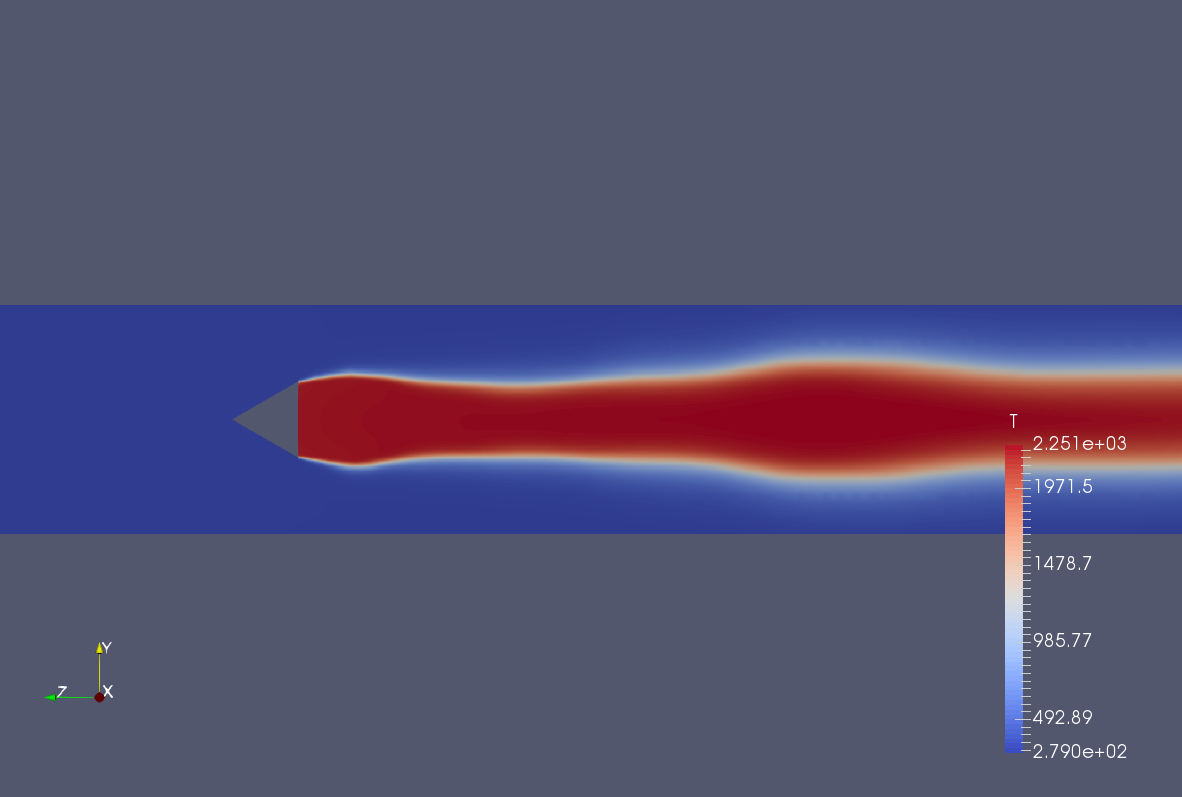
\includegraphics[width=\textwidth]{flame.png}
   \caption{Snapshot of temperature field in reacting flow case using GRI-Mech 3.0 and stock OpenFOAM solvers.}
   \label{F:flame}
  \end{subfigure}
  \caption{The bluff-body stabilized premixed turbulent flame simulation.}
\end{figure}




%% The Appendices part starts with the command \appendix;
%% appendix sections are then done as normal sections
\appendix
\setcounter{figure}{0}
\setcounter{table}{0}

% Fix for missing space between "Appendix" and letter
\renewcommand*{\thesection}{\appendixname~\Alph{section}}

\section{\texttt{pyJac}: analytical Jacobian generator for chemical kinetics}
\nociteS{Niemeyer:2016aa}
Accurate simulations of combustion phenomena require the use of detailed chemical kinetics in order to capture limit phenomena such as ignition and extinction as well as predict pollutant formation.
However, the chemical kinetic models for hydrocarbon fuels of practical interest typically have large numbers of species and reactions and exhibit high levels of mathematical stiffness in the governing differential equations, particularly for larger fuel molecules.
In order to integrate the stiff equations governing chemical kinetics, generally reactive-flow simulations rely on implicit algorithms that require frequent Jacobian matrix evaluations.
Some in situ and a posteriori computational diagnostics methods also require accurate Jacobian matrices, including computational singular perturbation and chemical explosive mode analysis.
Typically, finite differences numerically approximate these, but for larger chemical kinetic models this poses significant computational demands since the number of chemical source term evaluations scales with the square of species count.
Furthermore, existing analytical Jacobian tools do not optimize evaluations or support emerging SIMD processors such as GPUs.
Here we introduce \texttt{pyJac}, a Python-based open-source program that generates analytical Jacobian matrices for use in chemical kinetics modeling and analysis.
In addition to producing the necessary customized source code for evaluating reaction rates (including all modern reaction rate formulations), the chemical source terms, and the Jacobian matrix, \texttt{pyJac} uses an optimized evaluation order to minimize computational and memory operations.
As a demonstration, we first establish the correctness of the Jacobian matrices for kinetic models of hydrogen, methane, ethylene, and isopentanol oxidation (number of species ranging \numrange{13}{360}) by showing agreement within \SI{0.001}{\percent} of matrices obtained via automatic differentiation.
We then demonstrate the performance achievable on CPUs and GPUs using \texttt{pyJac} via matrix evaluation timing comparisons; the routines produced by \texttt{pyJac} outperformed first-order finite differences by \numrange{3}{7.5} times and the existing analytical Jacobian software \texttt{TChem} by \numrange{1.1}{2.2} times on a single-threaded basis.
It is noted that \texttt{TChem} is not thread-safe, while \texttt{pyJac} is easily parallelized, and hence can greatly outperform \texttt{TChem} on multicore CPUs.
The Jacobian matrix generator we describe here will be useful for reducing the cost of integrating chemical source terms with implicit algorithms in particular and algorithms that require an accurate Jacobian matrix in general.
Furthermore, the open-source release of the program and Python-based implementation will enable wide adoption.

\bibliographystyleS{unsrt}
\bibliographyS{prospectus}


\bibliographystyle{unsrt}
\bibliography{prospectus}

\end{document}
